\documentclass{beamer}

% There are many different themes available for Beamer. A comprehensive
% list with examples is given here:
% http://deic.uab.es/~iblanes/beamer_gallery/index_by_theme.html
% You can uncomment the themes below if you would like to use a different
% one:
%\usetheme{AnnArbor}
%\usetheme{Antibes}
%\usetheme{Bergen}
%\usetheme{Berkeley}
%\usetheme{Berlin}
%\usetheme{Boadilla}
%\usetheme{boxes}
%\usetheme{CambridgeUS}
%\usetheme{Copenhagen}
%\usetheme{Darmstadt}
%\usetheme{default}
%\usetheme{Frankfurt}
%\usetheme{Goettingen}
%\usetheme{Hannover}
%\usetheme{Ilmenau}
%\usetheme{JuanLesPins}
%\usetheme{Luebeck}
%\usetheme{Madrid}
%\usetheme{Malmoe}
%\usetheme{Marburg}
%\usetheme{Montpellier}
%\usetheme{PaloAlto}
%\usetheme{Pittsburgh}
%\usetheme{Rochester}
%\usetheme{Singapore}
%\usetheme{Szeged}
\usetheme{Warsaw}
%\usetheme{CambridgeUS}
%\usecolortheme{dolphin}
\usecolortheme{whale}

\addtobeamertemplate{navigation symbols}{}{%
	\usebeamerfont{footline}%
	\usebeamercolor[fg]{footline}%
	\hspace{1em}%
	\insertframenumber/\inserttotalframenumber
}

\title{Bodhitree}

\subtitle{E-learning platform development}

\author{Avijeet Gaikwad \\ 143050101}

\institute[] % (optional, but mostly needed)
{  Guided by \\
	\vspace{0.1cm}
	{\small Prof. Kameswari Chebrolu} \\
	and \\
	{\small Prof. Bhaskaran Raman} \\
	\vspace{0.5cm}
	Department of Computer Science and Engineering\\
  IIT Bombay}

\date{October 21, 2015}

\begin{document}

\begingroup
%\setbeamertemplate{headline}{}
\begin{frame}[plain]
  \titlepage
\end{frame}
\endgroup

\begin{frame}[allowframebreaks=0.9]{Outline}
  \tableofcontents
  % You might wish to add the option [pausesections]
\end{frame}

% Section and subsections will appear in the presentation overview
% and table of contents.
\section{Bodhitree and Multimedia Textbook}

\subsection{Bodhitree Introduction}

\begin{frame}{Bodhitree Introduction}{Components of the platform and introduction}
  \begin{itemize}
  \item {
    Small Private Online Courses (SPOCs)
  }
  \item {
    Bodhitree is an e-learning platform used to host SPOCs
  }
  \item {
  	Components of Bodhitree:
  	\begin{itemize}
  		\item Courseware
  		\begin{itemize}
  			\item Concepts
  			\item Discussion Forums
  			\item Assignments
  		\end{itemize}
  		\item Documents
  		\item Videos
  		\item Quizzes
  		\item ...
  	\end{itemize}
  }
  \end{itemize}
\end{frame}

\subsection*{Terminology}

\begin{frame}{Terminology}
	\begin{figure}
		\centering
		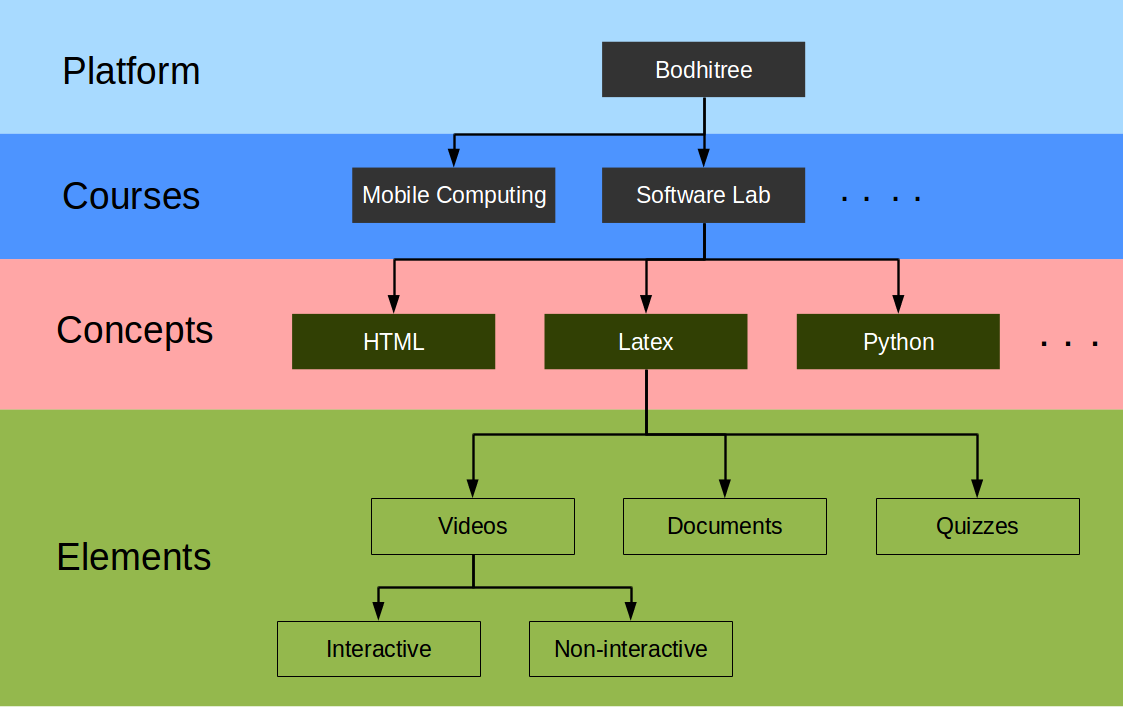
\includegraphics[width=0.8\linewidth]{media/bt}
		\caption{Components of Bodhitree and terminology}
		\label{fig:bt}
	\end{figure}

\end{frame}

\subsection{Multimedia Textbook}

\begin{frame}{Multimedia Textbook}
	\begin{figure}
		\centering
		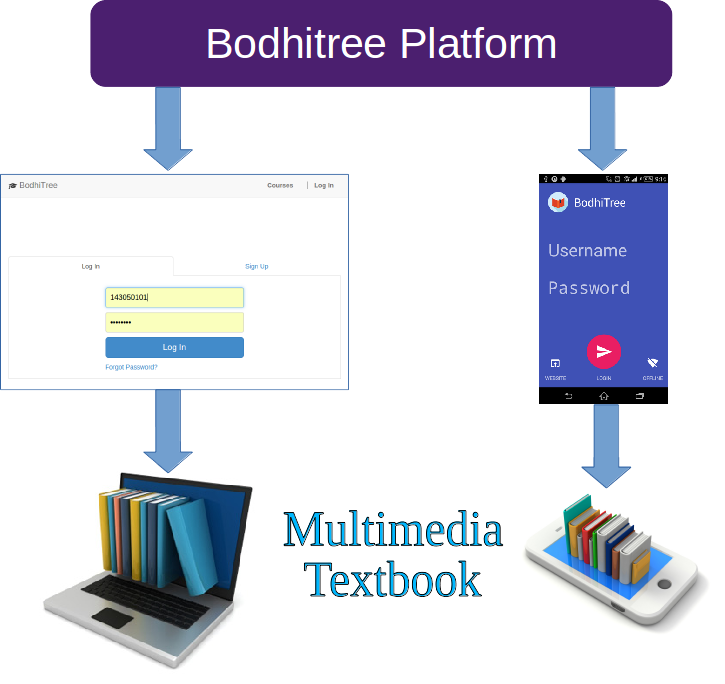
\includegraphics[width=0.6\linewidth]{media/bmmt}
		\label{fig:bmmt}
	\end{figure}
\end{frame}

\subsection{Additional Features}

\begin{frame}{Additional Features}
	\begin{itemize}
		\item \textbf{Access Control} %Users have different privileges to the content based on payment mode
		\item \textbf{Prerequisites Graph} %A suggested dependency/schedule map of the content that shows prerequisites to content
		\item Discussion section %Clarifying doubts with peers as well as instructor
		\item Student Progress Tracking
		\item Miscellaneous:
		\begin{itemize}
			\item Accounts misuse
			\item Server and client side logging
			\item Scalability
		\end{itemize}
	\end{itemize}
\end{frame}

\section{Access Control}

\begin{frame}{Access Control}{Differential access to content based on payment}
	\begin{figure}
	\centering
	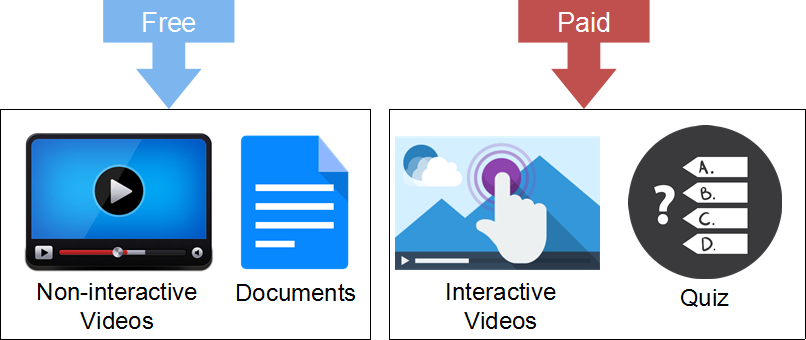
\includegraphics[width=0.7\linewidth]{media/AccessControl}
	\label{fig:AccessControl}
	\end{figure}
\end{frame}

\subsection{Problem Statement}

\begin{frame}{Access Control}
	\begin{block}{Problem Statement}
		\begin{itemize}
			\item Paid content in the multimedia textbook
			\item Content developer needs to have control over what content is accessible to the students
		\end{itemize}
	\end{block}
\end{frame}

\subsection{Specifications}

\begin{frame}{Specifications}
	\begin{itemize}
		\item Tagging of concept elements by the content developer, elements being any of the following:
		\begin{itemize}
			\item Videos
			\item Documents
			\item Quizzes
			\item Video markers
		\end{itemize}
		\item There are 5 fixed tags \textit{(P1, P2, P3, P4 and P5)}, and the default tag is \textit{Free}
		\item Content developer can add custom tags
		\item These tagged elements cannot be accessed by the students having the default
		access to Bodhitree, i.e. students having access only to the free content
	\end{itemize}
\end{frame}

%\begin{frame}{Specifications}
%	\begin{itemize}
%		\item Tagging of concept elements by the content developer, elements being any of the following:
%		\begin{itemize}
%			\item Videos
%			\item Documents
%			\item Quizzes
%			\item Video markers
%		\end{itemize}
%		\item By default, the elements are free. Once tagged, they require special privilege to be accessed
%		\item Content developer can provide access to students
%	\end{itemize}
%\end{frame}

\subsection{System Design}

\begin{frame}{Design}
	\begin{figure}
	\centering
	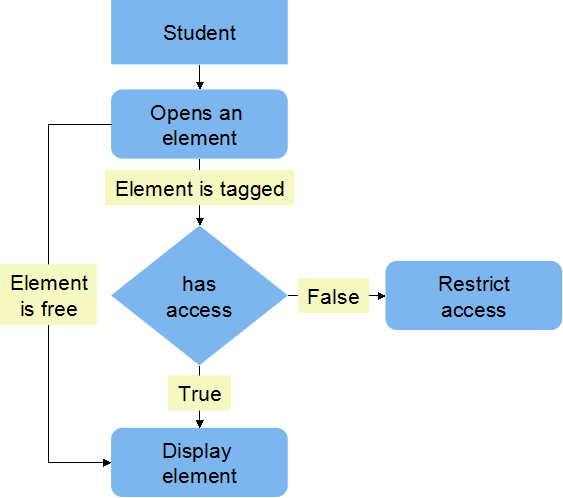
\includegraphics[width=0.6\linewidth]{media/ACdfd}
	\label{fig:ACdfd}
	\end{figure}
\end{frame}

\begin{frame}{Tagging}
	\begin{itemize}
		\item 5 fixed tags \textit{(P1, P2, P3, P4, P5)}, default is \textit{Free}
		\item Content developer can add custom tags
		\item Grouping of access by using tags
	\end{itemize}
	
\end{frame}

\begin{frame}{Users access to content}
	\begin{itemize}
		\item By default, users have access to the \textit{Free} content. Content developer has the authority to grant access to tagged content
		\item Users can see the title and the link for all elements
		\item Interactive videos are shown as plain videos to unauthorized users
	\end{itemize}
	
\end{frame}

\begin{frame}{Granting access to users}
	\begin{itemize}
		\item Uploading the CSV file:
		\begin{center}
		\begin{tabular}{|c|c|c|c|}
			\hline stud1 & P1 & P2 & P3 \\ 
			\hline stud2 & P1 &  &  \\ 
			\hline stud3 & P3 &  &  \\ 
			\hline 
		\end{tabular}
		\end{center} 
		\item Checking username against the registered users
		\item Storing the tags in the database: 
		\begin{center}
			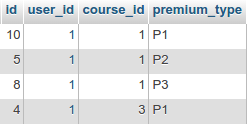
\includegraphics[width=0.5\linewidth]{media/premiumAccesses}
		\end{center}
	\end{itemize}
\end{frame}

\begin{frame}
	Interface to upload the CSV file:
\begin{figure}
\centering
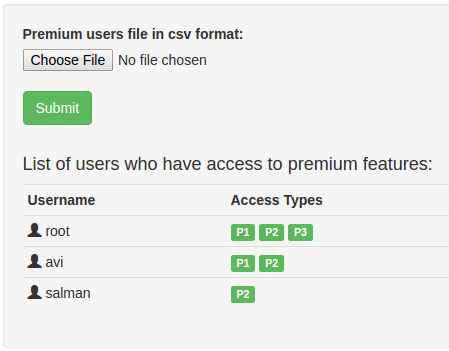
\includegraphics[width=0.8\linewidth]{media/CSVupload}
\label{fig:CSVupload}
\end{figure}
\end{frame}

\begin{frame}
	Information displayed after an upload
	\begin{figure}
	\centering
	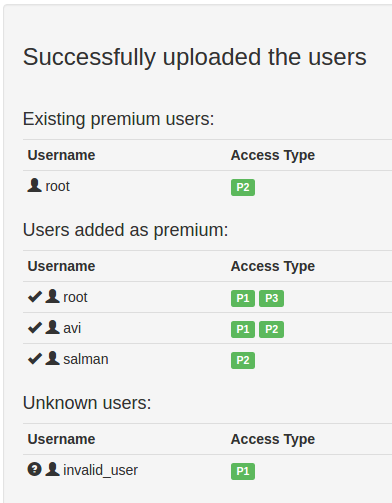
\includegraphics[width=0.7\linewidth]{media/usertaguploadsuccess}
	\label{fig:usertaguploadsuccess}
	\end{figure}
\end{frame}

\begin{frame}{Removing of tags access from users}
	\begin{itemize}
		\item Content developer has the authority to remove the tags access
		\item Checklist provided listing the users and associated tags
		\item Corresponding entries removed from the database
	\end{itemize}
\end{frame}

\begin{frame}
	Interface to remove tag access
	\begin{figure}
	\centering
	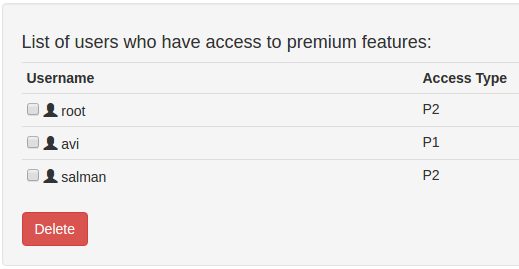
\includegraphics[width=0.8\linewidth]{media/removeusers}
	\label{fig:removeusers}
	\end{figure}
\end{frame}

\subsection{Implementation}

\begin{frame}{Implementation}
	\begin{itemize}
		\item When a user opens a concept page, the tags he has access to are checked from the premiumuser table
		\item Data fetched according to the access
		\item Key value pair \textit{has\_access} generated which helps in rendering the component at the client side
	\end{itemize}
\end{frame}

\begin{frame}{Data sent to client who is not having access to an element}	
	\begin{figure}
	\centering
	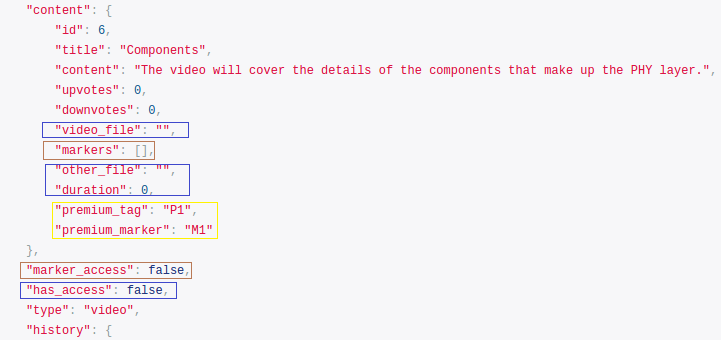
\includegraphics[width=1\linewidth]{media/SUgetdata}
	\label{fig:SUgetdata}
	\end{figure}
\end{frame}

\begin{frame}{Tagging interface for the content developer}
	\begin{center}
		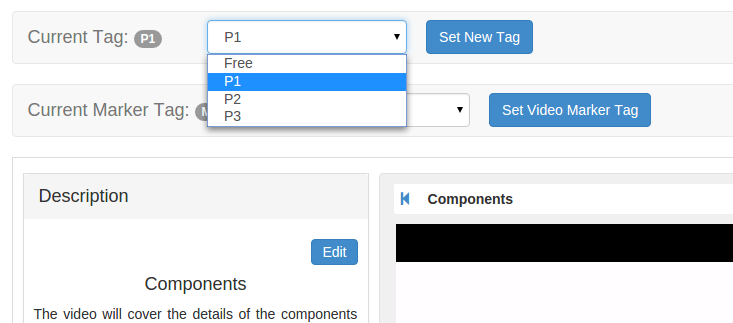
\includegraphics[width=1\linewidth]{media/tagging_interface}
	\end{center}
\end{frame}

\begin{frame}{User's view of unauthorized access}
	\begin{center}
		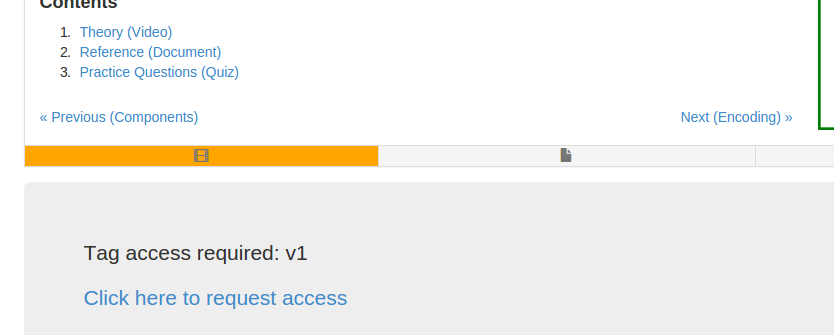
\includegraphics[width=1\linewidth]{media/sAccessNot}
	\end{center}
\end{frame}

\section{Prerequisites Graph}

\begin{frame}{Prerequisites Graph}
	\begin{figure}
		\centering
		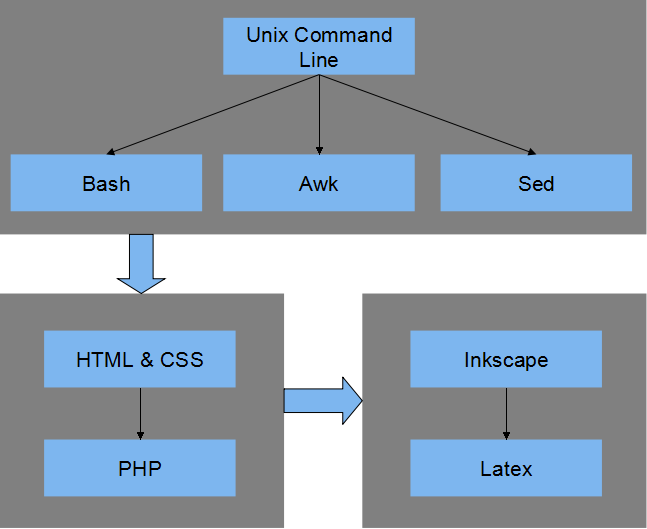
\includegraphics[width=0.7\linewidth]{media/prereq-graph}
		\label{fig:prereq-graph-calc}
	\end{figure}
\end{frame}

\subsection{Problem Statement}

\begin{frame}{Prerequisites Graph}
	\begin{block}{Problem Statement}
		\begin{itemize}
			\item Map the relations between concepts and display a guideline to proceed in a course
			\item Display link to prerequisites on the concept page for easy navigation
		\end{itemize}
	\end{block}
\end{frame}

\subsection{Specifications}

\begin{frame}{Specifications}
	\begin{itemize}
		\item Content developer specifies the prerequisites
		\item Initial graph generated automatically, content developer can modify and then finalize it
		\item The final graph shown to the students acts as a guideline to proceed in the course
	\end{itemize}
\end{frame}

\subsection{Design and Implementation}

\begin{frame}{Design and Implementation}
	\begin{itemize}
		\item Prerequisites stored as a list of concept id's
		\item Prerequisites are retrieved when the user opens a concept page, links are provided
		\begin{figure}
			\centering
			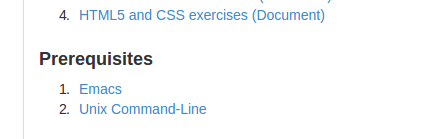
\includegraphics[width=0.8\linewidth]{media/PrereqList}
			\caption{Snap of prerequisites displayed on a concept page}
			\label{fig:PrereqList}
		\end{figure}
	\end{itemize}
\end{frame}

\begin{frame}
	Several graph generation libraries used to generate initial graphs:
	\begin{itemize}
		\item \textbf{Graphviz:} Python library which generates an image of the final graph, non-interactive
		\item \textbf{Arbor.js:} Javascript library which dynamically generates interactive graphs, allows users to interact with the components
		\item \textbf{GoJS:} Allowed the creation of a graph which the content developer can modify
	\end{itemize}
\end{frame}

\begin{frame}{Graphviz}
	\begin{figure}
		\centering
		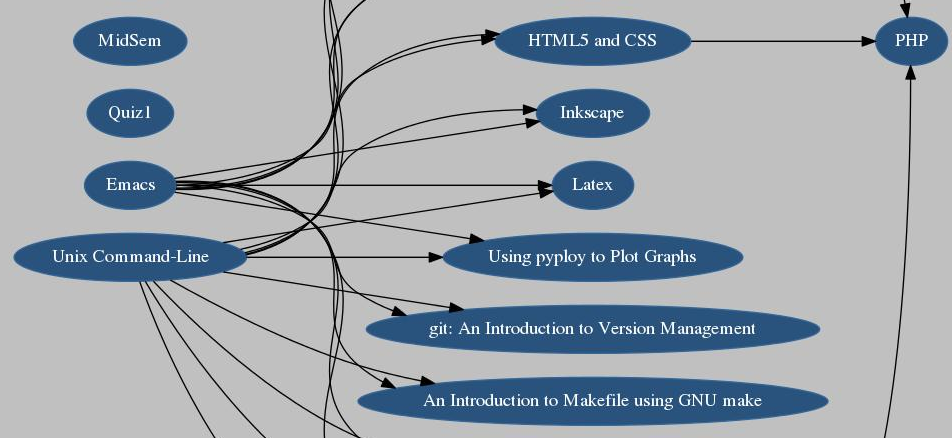
\includegraphics[width=0.8\linewidth]{media/Graphviz}
		\caption{Part of a complex graph generated using graphviz}
		\label{fig:Graphviz}
	\end{figure}
\end{frame}

\begin{frame}{Arbor.js}
	\begin{figure}
		\centering
		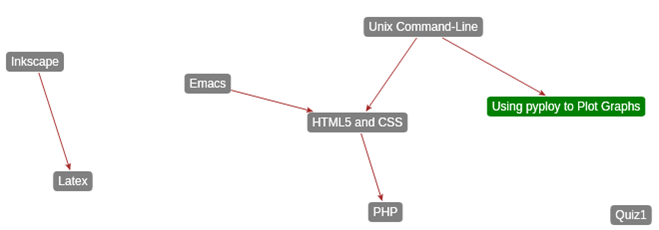
\includegraphics[width=0.8\linewidth]{media/PrereqGraph}
		\caption{Part of a graph generated using arbor.js}
		\label{fig:PrereqGraph}
	\end{figure}
\end{frame}

\section[]{Conclusion}

\section{Marks Module}

\subsection{Problem Statement}

\begin{frame}{Marks module}{Store and display students marks}
	\begin{block}{Problem Statement}
		\begin{itemize}
			\item Store student’s marks on Bodhitree
			\item Enable the students to view their marks on the course page
		\end{itemize}
	\end{block}
\end{frame}

\subsection{Specifications}

\begin{frame}{Specifications}
	\begin{itemize}
		\item The instructor can upload a CSV file containing the marks of the students
		\item Student can log into his Bodhitree account and can see his marks on the course page
	\end{itemize}
\end{frame}

\subsection{Design}

\begin{frame}{Design}
	\begin{itemize}
		\item CSV file upload and storing the marks
		\item Displaying marks to the user
		\item Handling authorization
	\end{itemize}
\end{frame}

\begin{frame}
	Required format of the CSV file: \\
	\vspace{0.4cm}
	%	\begin{itemize}
	%		\item First line is the names of exams
	%		\item Second line is the maximum marks of that exam
	%		\item The lines that follow are the usernames of students followed by their marks
	%	\end{itemize}
	\centering
	\begin{tabular}{|c|c|c|c|c|}
		\hline \rule[-2ex]{0pt}{5.5ex} EXAM\_TYPE & Q1 & Midsem & Q2 & Endsem \\ 
		\hline \rule[-2ex]{0pt}{5.5ex} MAX\_MARKS & 20 & 30 & 20 & 30 \\ 
		\hline \rule[-2ex]{0pt}{5.5ex} Student 1 & 18 & 25 & 12 & 22 \\ 
		\hline \rule[-2ex]{0pt}{5.5ex} Student 2 & 12 & 20 & 14 & 24 \\ 
		\hline \rule[-2ex]{0pt}{5.5ex} Student 3 & 16 & 24 & 0 & 22 \\ 
		\hline 
	\end{tabular} 
\end{frame}

\begin{frame}{Snapshot of the tables involved in the marks module}
	\begin{figure}
		\centering
		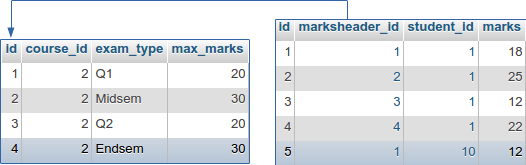
\includegraphics[width=0.8\linewidth]{media/marksdb} \\
		Marks Header \hspace{2cm} Students Marks
		\caption{Database schema of the marks module}
		\label{fig:marksdb}
	\end{figure}
	
\end{frame}

\begin{frame}{Instructor's view}
	\begin{figure}
		\centering
		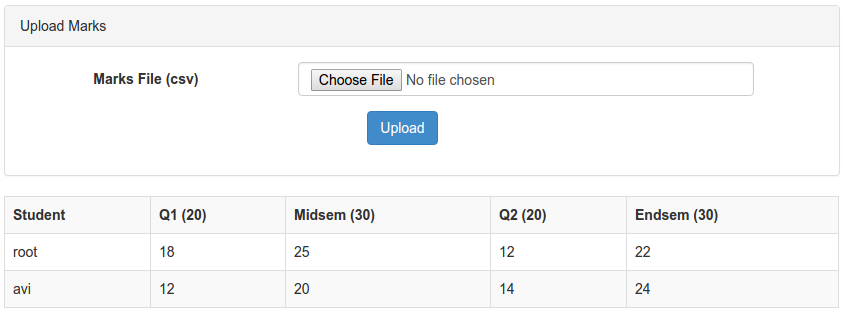
\includegraphics[width=0.8\linewidth]{media/marksi}
		\caption{Instructor's view of CSV upload and display of students marks}
		\label{fig:marksi}
	\end{figure}
\end{frame}

\begin{frame}{Student's view}
	\begin{figure}
		\centering
		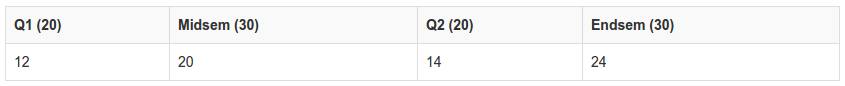
\includegraphics[width=0.8\linewidth]{media/markss1}
		\caption{Student 2's view of his marks}
		\label{fig:markss1}
	\end{figure}
\end{frame}

\begin{frame}{Conclusion}
	\begin{itemize}
		\item Work on the marks module is done, thoroughly tested
		\item Access control module is implemented, initial testing done
		\item Some changes are suggested for the access control module
		\begin{itemize}
			\item Changing of certain information text displayed to users
			\item List of users who have premium access must collate
			\item ...
		\end{itemize}
		\item Specifications for prerequisites graph module are set
		\begin{itemize}
			\item Certain initial graphs are implemented
			\item Interactivity to content developer is needed
			\item Thinking about interactivity to students
		\end{itemize}
	\end{itemize}
\end{frame}

\begin{frame}
	\centering
	\huge
	Thank you!
\end{frame}

\end{document}